\documentclass[conference]{IEEEtran}

\usepackage{tikz}
\usepackage{graphicx}
\usepackage{amssymb,amsmath,amsfonts,amsthm}

\newtheorem{theorem}{Theorem}
\newtheorem{lemma}[theorem]{Lemma}
\newtheorem{proposition}[theorem]{Proposition}
\newtheorem{corollary}[theorem]{Corollary}

\theoremstyle{definition}
\newtheorem{definition}{Definition}
\newtheorem{example}{Example}
\newtheorem{observation}{Observation}


\begin{document}

\title{Forward-Engineering MAC: Energy Efficiency and Resource Accounting}

\author{\authorblockN{Gareth B. Middleton and David T.-H. Kao}
\authorblockA{Rice University}}

\maketitle

\begin{abstract}

Progress Report for ELEC 537 (Fall 2007) Project
November 8th, 2007

\end{abstract}

\section{Introduction}

The distributed nature of many medium access control (MAC) protocols is very amenable to game theoretic analysis \cite{LTHCC07,XSR05}. Recently, this has resulted in reverse engineering of the 802.11 MAC in a non-cooperative context \cite{LTHCC07}, with the aim of discovering what utility function the 802.11 MAC best implements. By approximating the 802.11 distributed coordination function
(DCF) as a time-slotted system where users have adjustable probabilites of transmission, the authors demonstrate that nodes are in fact taking part in a game where each has an individually defined utility. Furthermore, the authors propose game-playing dynamics that ensure convergence under mild conditions.

Further extensions of this work have focused primarily on fairness and efficiency in the context of Network Utility Maximization \cite{LCC07}. By defining individual utility functions proportional to some network-wide utility, and with the use of limited message passing, MAC protocols were developed that can converge to game-theoritically optimal solutions.

In this work, we take the approach of \emph{forward} engineering a protocol from game-theoretic foundations. Rather than defining our utility functions in terms of an existing MAC, we attack the problem of taking practical considerations existing at each node into account when crafting our utility function. Taking this approach, we succesfully define a function capturing the selfish nature of each node.

This progress report describes our utility function, the considerations giving rise to its definition, and simulation results showing the behavior of a network implementing such a function. In the final version of this work, we will address the issue of making the persistence probability well-known, i.e. we will account for the overhead associated with implementing MAC games in practice.

\section{Preliminaries}
\subsection{Game Theory Background}
Our analysis in this project hinges on a number of fundamental concepts from noncooperative game theory. We review here a number of these fundamentals, but refer the reader to \cite{OsborneRubinstein_book} for a more complete and rigorous presentation. 

A noncooperative {\em Game} in normal form consists of three ingredients:
\begin{itemize}
	\item A set of players
	\item For each player, a set of feasible strategies 
	\item For each player, a utility function that is a function of the collection of strategies played by all players.
\end{itemize}

For the remainder of this report we use $i \in C$ as the index of a given player (where $C = \{1,\ldots,N\}$). We also use $p_i$ to represent a strategy of Player $i$, and $p_{-i}$ to represent the strategy profile of all players besides $i$. Finally we denote the utility of Player $i$ as $u_i$.

A Nash equilibrium then is a strategy profile where no player may increase its utility by deviating from its equilibrium strategy, i.e.
\begin{eqnarray}
	\lefteqn{u_i(p_i^\star,p_{-i}^\star) \geq u_i(p_i,p_{-i}^\star)}\nonumber \\
	& & \forall p_i\in[p_i^{MIN},p_i^{MAX}], \ i \in C.
\end{eqnarray}
From an engineering viewpoint then, a Nash Equilibrium has a number of desirable characteristics that describe the steady state of a distributed system.

Convergence of a particular dynamic, or way to play the game, is largely dependent on the game at hand. However, we confine our study to utility functions that are of the class $C_1$ (i.e. continuous and differentiable) and quasi-convex. This will ensure convergence of the two most common dynamics: best-reply and gradient play.

\subsection{Prior Work}
The reverse-engineering of 802.11 MAC as a noncooperative game was presented recently in \cite{LTHCC07}. Based on specifications in the standard, the authors discovered that the utility function of a wireless user was in fact
\begin{eqnarray}
	u_i(p_i,p_{-i}) &=& p_i^2\left(\frac{1}{4} - \frac{1}{3}p_i\right)\prod_{j \in C\setminus i}(1-p_j)\nonumber \\
	& & -\frac{1}{6}p_i^2\left(1 - \prod_{j \in C\setminus i}(1-p_j)\right).
	\label{eq:rem}
\end{eqnarray}

We believe while this contribution is very significant, it raises questions regarding the design of the 802.11 MAC. This definition does not particularly represent any concrete concept of utility and in fact seems to be a method of loosely introducing cooperation into the system. Since the contention of the medium is somewhat antagonistic, this cooperation actually improves performance all around. An open question then is, ``Are there other definitions of utility that may further a more specific goal?``. To that effect, in \cite{LCC07} a fairness objective was considered where all of the users shared an identical utility function. In our work, we consider another possible definition of utility that is both intuitive and yet still reflects the selfish nature of noncooperative users.

\subsection{Medium Access Contention Games}
Our system model is largely based the one described in \cite{LTHCC07}. Consider a single-clique topology containing $N$ individual single-hop flows. Each flow, or user, is indexed by a value $i$ where
\begin{equation}
	i \in C, \ \ C = \{1,\ldots,N\}.
\end{equation}

Users access the medium during time slots each with a persistence probability $p_i$; this models the RTS/CTS phase of 802.11. For each user this persistence probability can change over time, however it must lie within a specified interval: $[p_i^{MIN},p_i^{MAX}]$. In the event of multiple users simultaneously accessing the channel, a collision occurs, thus only one user may use the channel at a given time. 

Under the non-cooperative framework devised, each User~$i$ is a player of a game, where the strategy and strategy set are the persistence probability $p_i$ and the set of permissible persistence probabilities respectively. The remaining ingredient to define any non-cooperative game is a set of individual utility functions decribing payoffs given the set of user strategies. We discuss this in the following section. For the remainder of this work we call this class of games Medium Access Control (MAC) Games.


\section{Defining a Utility Function}
\subsection{Bad Definitions of Utility}
Considering an arbitrary wireless node, we note that the key factor which relates to user experience is throughput. Let $p_i$ be the ``persistence probability'' of User~$i$. In the network previously described then, the throughput $s_i$ of User~$i$ with packet length $L$ is given by
\begin{eqnarray}
	s_i & \triangleq & L p_i Pr[\text{no collision}] \nonumber \\
		& = & L p_i \prod_{\substack{j \in C\\j \neq i}} (1-p_j). \label{eq:thru}
\end{eqnarray}
We now describe a class of utility functions that result in possibly degenerate networks. 
\begin{definition}[Bad Utility Functions]
	We call a MAC game {\em bad} if the definition of utility for each user is such that for a User~i
	\begin{equation}
		u_i(p_i^{MAX},p_{-i}) \geq u_i(p_i,p_{-i}), \ \ \forall p_i\in[p_i^{MIN},p_i^{MAX}].
	\end{equation}
\end{definition}

The justification for this definition is that if $p_i^{MAX} = 1$ for any User~$i$, the game degenerates into a situation where either one or zero users experience any throughput. In addition to being academically uninteresting, this sort of situation is what most system designers would hope to avoid. 
\begin{observation}
	Any MAC game where the utility functions for all users, $u_i(p_i)$, is monotonically increasing with $p_i$ is bad.
\end{observation}
Notice that this classifies throughput, $s_i$, as a bad definition for utility. This also explains to some degree the reverse-engineered utility of (\ref{eq:rem}); the engineers who originally designed the exponential backoff approach to medium access were, in some sense, artificially incorporating a cooperative element in a selfish utility, thus improving overall system performance.

\subsection{Smiles per Watt}
Generally speaking, a user with more throughput will be happier than one with less. However the degree of satisfaction is tempered by the demands of a particular application. Additionally, power management is an issue of great inportance in mobile wireless devices. To this end, we define a quality of service (QoS) based utility function that also considers the energy expended to achieve that level of satisfaction.

We will first define a function which represents the user's QoS.  We require that, as a function of throughput, the QoS should be
monotone increasing, and should be zero for zero throughput.  We also require that the function reach some maximal value as a throughput goes to infinity; consider a user watching a streaming video--at some point, more throughput does not improve the experience.  With these requirements in mind, we propose the following QoS function:
\begin{equation}
  Q_i(s_i) \triangleq M \left(\frac{\tanh\left[As-s_0\right] - \tanh\left[-s_0\right]}{1-\tanh\left[-s_0\right]}\right).
  \label{eq:qos1}
\end{equation}
where the constants $M, A, s_0 > 0$ are scaling and shifting values affecting the shape of the curve, which can be adapted to the service being considered. Of these, the parameter $A$ conveys the most about User $i$'s throughput demand. As $A$ increases, the $Q_i$ is compressed and User $i$ becomes satisfied at a lower rate. We have plotted an example of the QoS function in Figure \ref{fig:QoS}. Notice that all of our requirements above are met by the hyperbolic tangent function. By substitution of (\ref{eq:thru}) we arrive at the QoS as a function of the persistence probability $p_i$.
\begin{eqnarray}
  \lefteqn{Q_i(p_i) \triangleq}\nonumber\\
  & M \left(\frac{\tanh\left[A\left(L p_i \prod_{\substack{j \in C\\j \neq i}} (1-p_j)\right)-s_0\right] - \tanh\left[-s_0\right]}{1-\tanh\left[-s_0\right]}\right)
\end{eqnarray}

Noting that mobile wireless devices are ultimately constrained by battery power (which diminishes over time), we must scale the user satisfaction by a penalty term reflecting energy use.  Intuitively, this corresponds to a user consuming excess bandwidth, but then becoming ``disappointed'' when the device fails due to low battery after a short time. Thus we arrive at our utility function:
\begin{equation}
  u_i(p_i) \equiv \frac{Q_i(p_i)}{kp_i},
  \label{eq:util}
\end{equation}
where $k$ represents a scaling constant on battery drain.  The units of $u_i$ can be thought of as energy efficient satisfaction or ``smiles per watt.'' A plot demonstrating typical characteristics of $u_i(p_i)$ appears in Figure \ref{fig:QoS}.  A key feature of this function is its well-defined peak.

%\usepackage{graphics} is needed for \includegraphics
\begin{figure}[htp]
\begin{center}
\begin{tikzpicture}[domain=0:1, xscale=6, yscale=3, samples=50]
\draw[help lines,xstep=0.2,ystep=.5 ] (0,0) grid (1,1.5);
\draw[-latex] (-0.03,0) -- (1.03,0) node[right] {$p$};
\draw[-latex] (0,-.05) -- (0,1.65) node[above] {$Q(p)$};
 
 \foreach \t in {.2,.4,.6,.8,1}{\draw (\t,.01) -- (\t,-.01) node[below] {$\t$};}
 \draw[red, smooth, thick] plot file{document.qos.table} node [right, below] {$Q(p)$};
 \draw[blue, smooth, thick] plot file{document.u.table} node [right,above] {$u(p)$};

%\draw[color=red]plot[id=qos]function{(tanh(5*(x-.5))-tanh(5*(0-.5)))/(1-tanh(5*(0-.5)))};
%\draw[color=blue]plot[id=u]function{(tanh(5*(x-.5))-tanh(5*(0-.5)))/(x*(1-tanh(5*(0-.5))))};
\end{tikzpicture}
\caption{some Caption}
\label{fig:QoS}
\end{center}
\end{figure}

\section{Simulation Results}
\subsection{System Configuration}
All simulations in the following presentation were performed via Matlab. Discovery of Nash Equilibria was accomplished via gradient play, and comparisons with the 802.11 utility function assumed a $p_i^{MAX}$ of one half (a two-slot minimum contention window) and binary exponential backoff. 

\subsection{General Performance}
In our first simulation we investigated the actual behavior of the new utility function (\ref{eq:util}). We illustrate here the differences in the result of the game when a two user network is symmetric (both users have identically defined utilities) and asymmetric (differently defined utilities. The differences in utility are accomplished by varying the $A$ parameter as this relates to the level of satisfaction a user receives at a given level of throughput.
\begin{figure}[htp]
\begin{center}
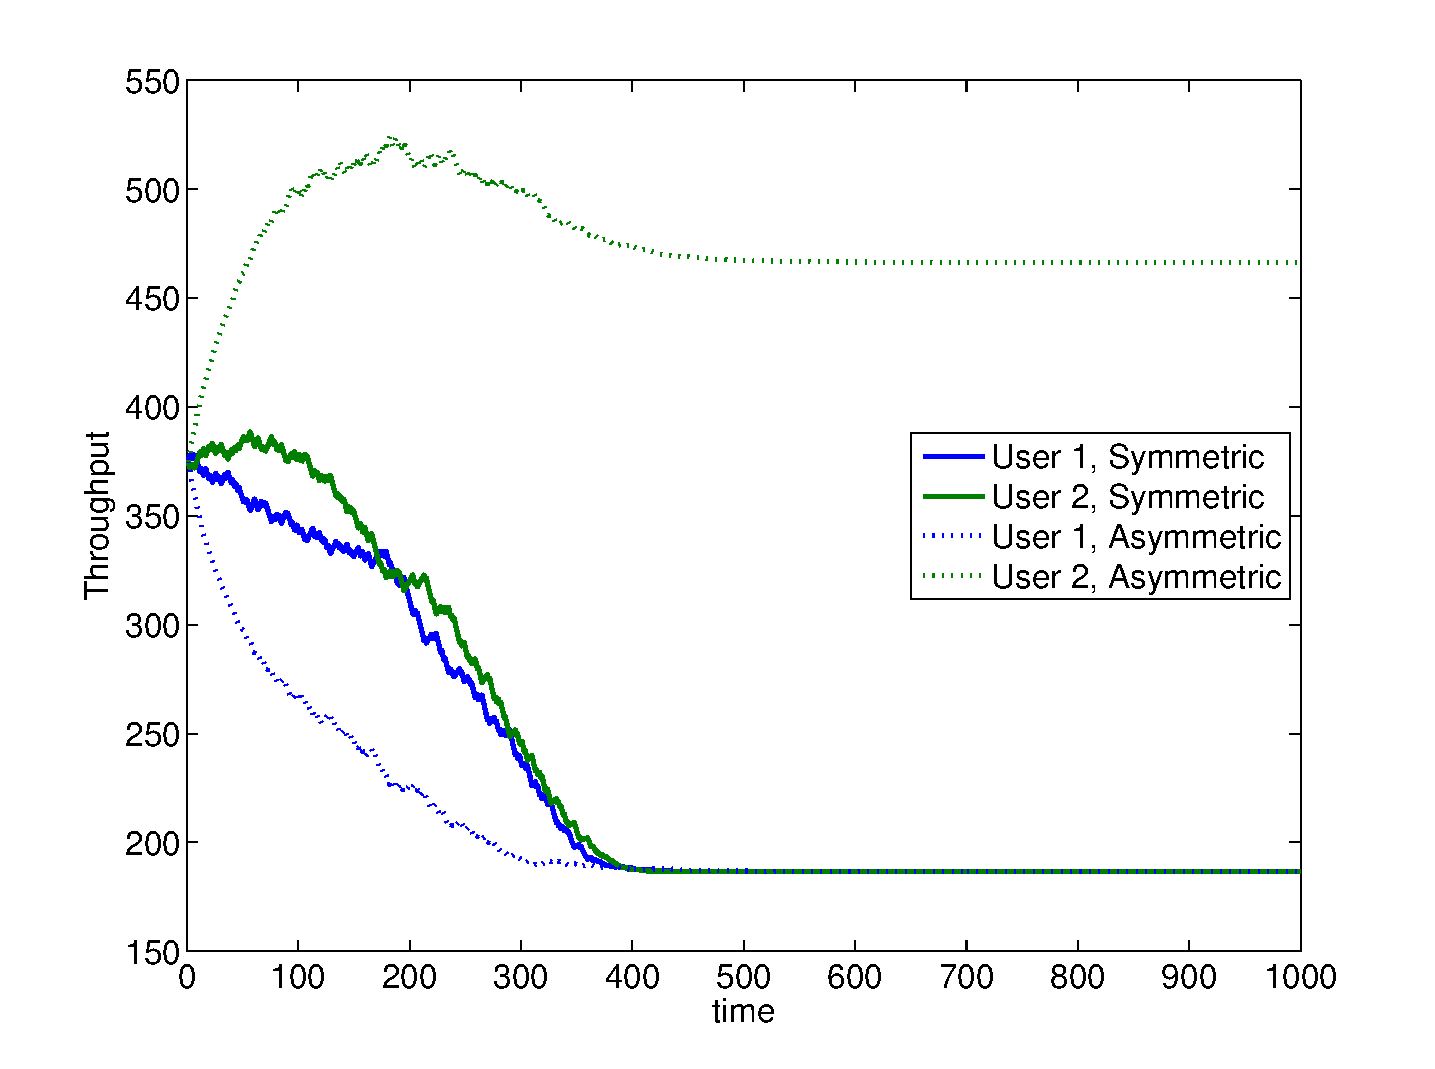
\includegraphics[width=3in]{sim1a.pdf}
\caption{Evolution of Throughput for two-node symmetric and asymmetric networks}
\label{fig:sim1a}
\end{center}
%
\end{figure}
\begin{figure}[htp]
\begin{center}
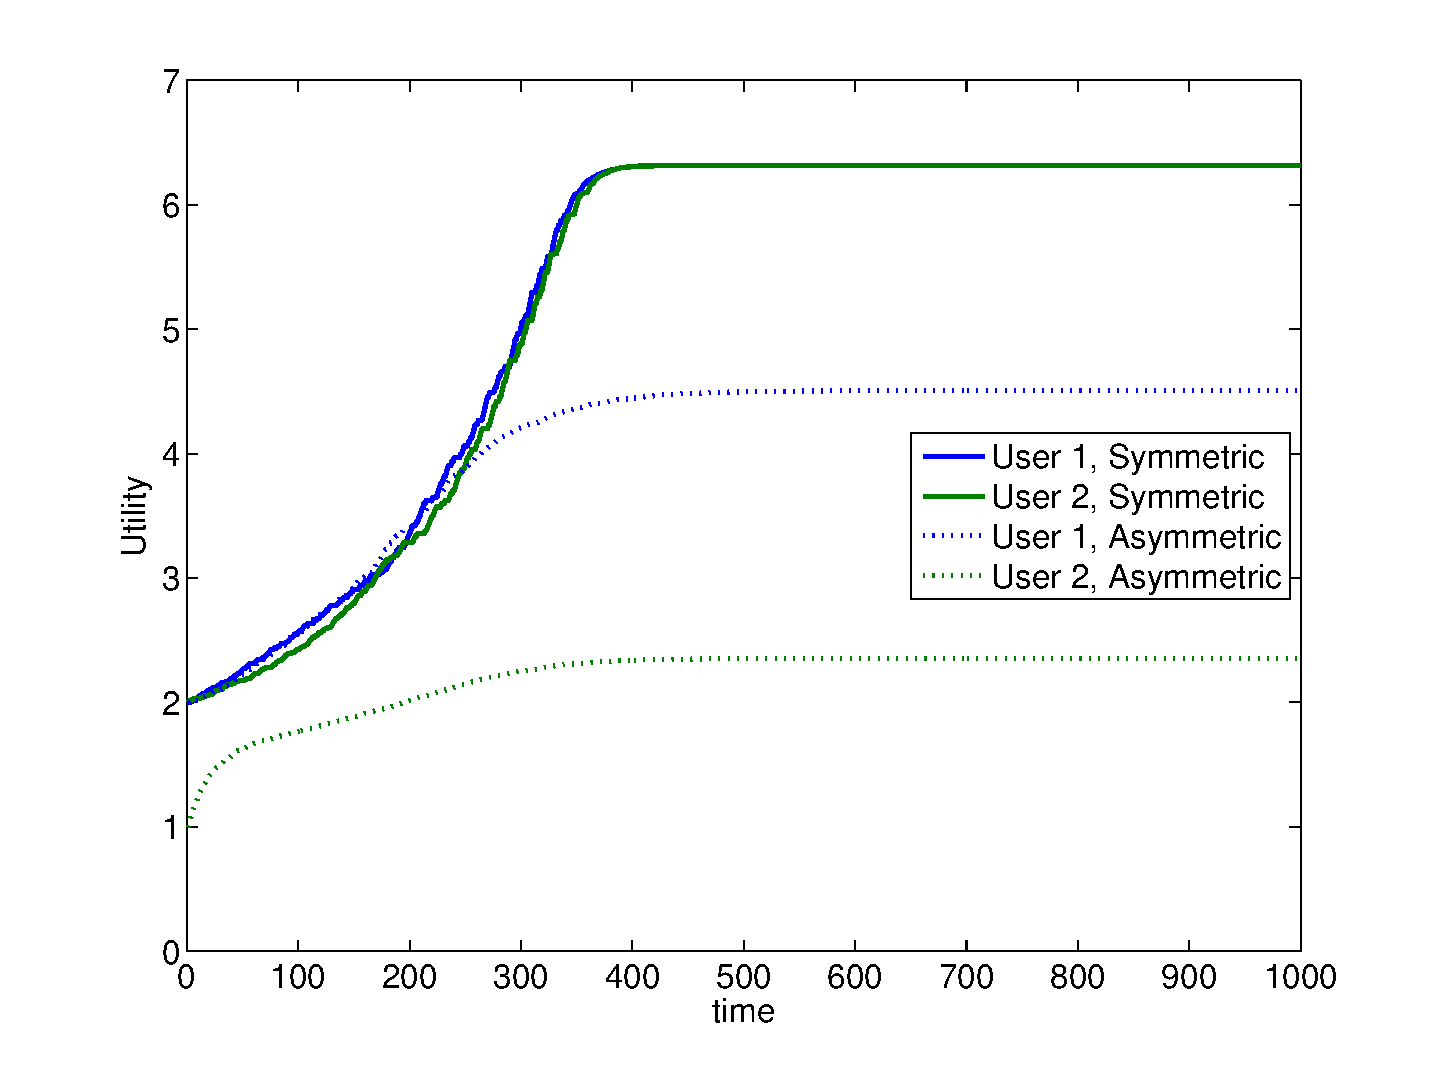
\includegraphics[width=3in]{sim1b.pdf}
\caption{Evolution of Efficient QoS Utility for for two-node symmetric and asymmetric networks}
\label{fig:sim1b}
\end{center}
\end{figure}
%
\begin{figure}[htp]
\begin{center}
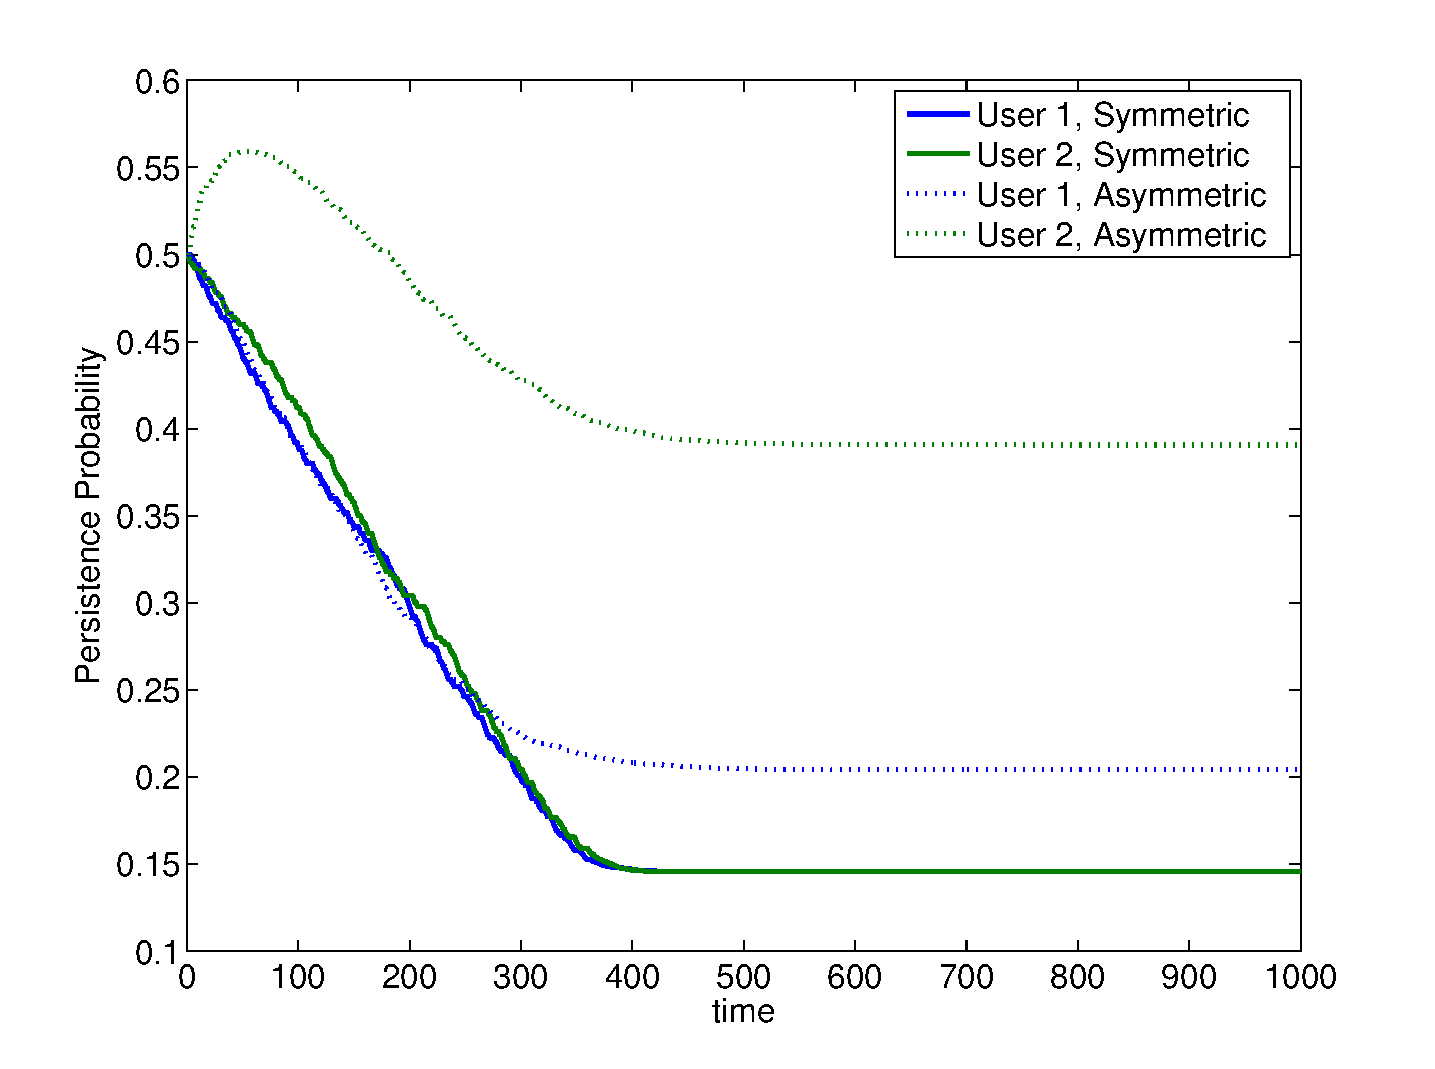
\includegraphics[width=3in]{sim1c.pdf}
\caption{Evolution of Persistence Probabilities (Strategies) for two-node symmetric and asymmetric networks}
\label{fig:sim1c}
\end{center}
\end{figure}
Figures \ref{fig:sim1a}-\ref{fig:sim1c} demonstrate differences between symmetric and asymmetric definitions regarding how the throughput, user utility and persistence probability vary as users play the game. In the asymmetric network User 2 had a utility defined such that it was more demanding of throughput (lower $A$). This affected the system overall in a number of ways. First, the Nash Equilibrium point of the asymmetric network results in User 2 receiving more throughput than User 1. This was accomplished by more aggressively accessing the medium, as demonstrated by the higher equilibrium persistence probability. Additionally, although User 1 received roughly the same throughput at equilibrium in both symmetric and asymmetric scenarios, it needed to expend more energy to do so and thus its utility was lower in the assymetric case.



\subsection{Comparison with 802.11}
In this section we compare the performance of our utility function with that of the 802.11 definition. We confined our simulations here to symmetric networks of five users, and examine average user throughput, QoS and QoS-per-Watt at equilibrium as a function of the parameter $A$. Remember that this parameter governs how easily satisfied a user is at a given level of throughput. For smaller values of $A$ the users demand more throughput, whereas for larger values users are easily satisfied by nominal rates.
\begin{figure}[htp]
\begin{center}
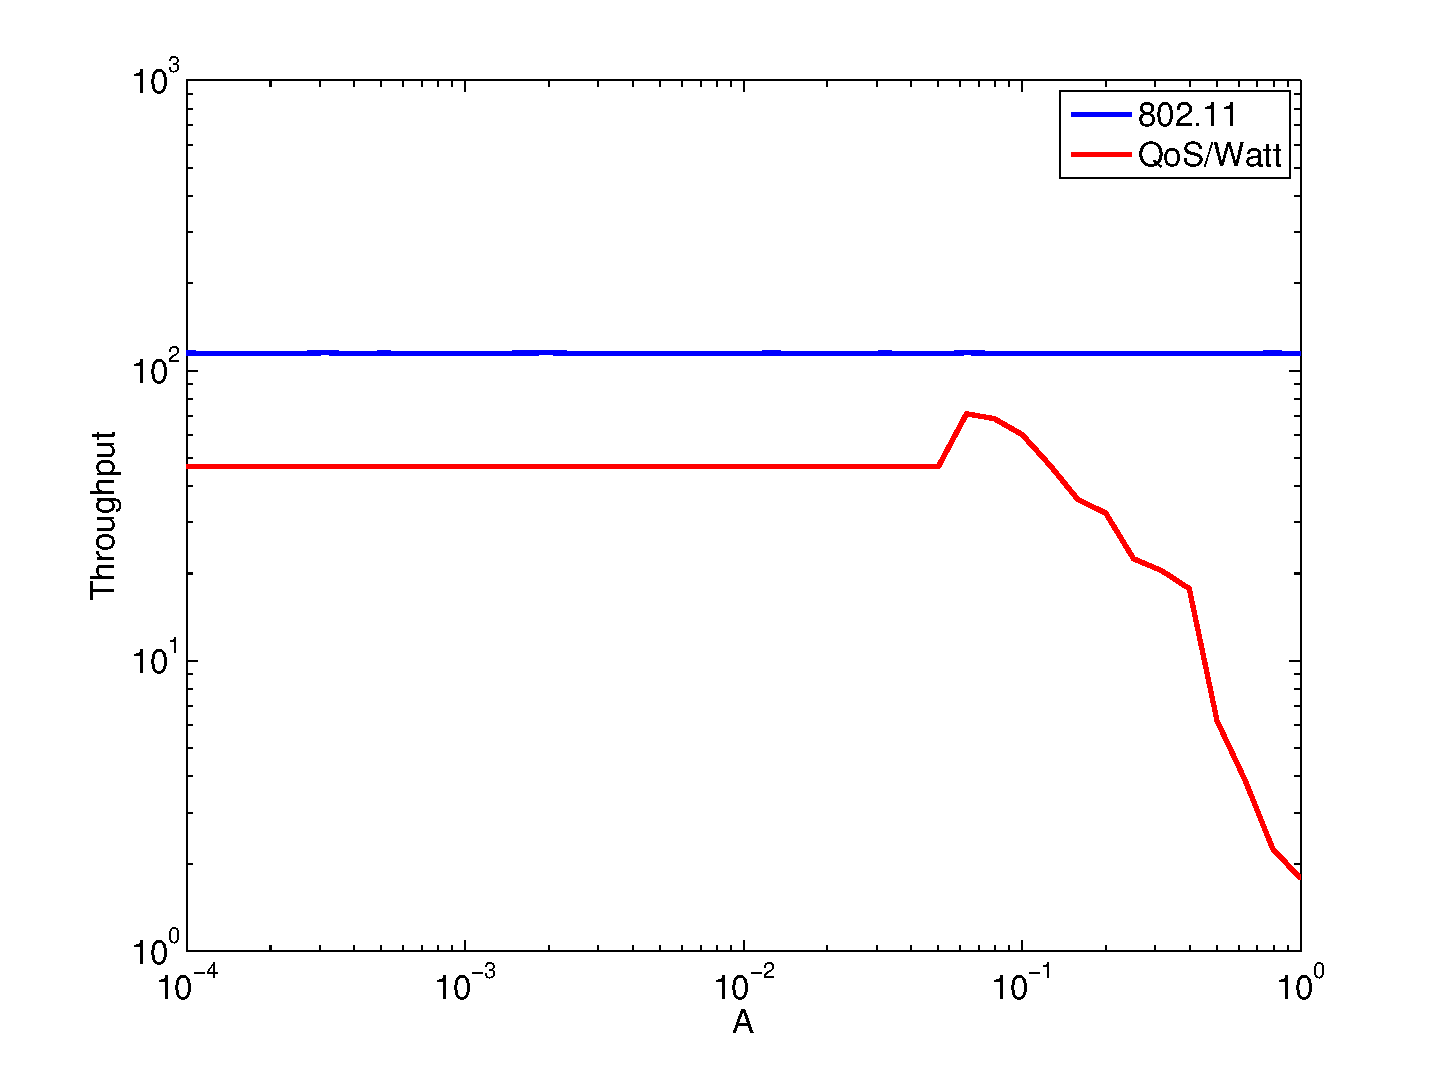
\includegraphics[width=3in]{sim2a.pdf}
\caption{Throughput vs. A}
\label{fig:sim2a}
\end{center}
%
\end{figure}
\begin{figure}[htp]
\begin{center}
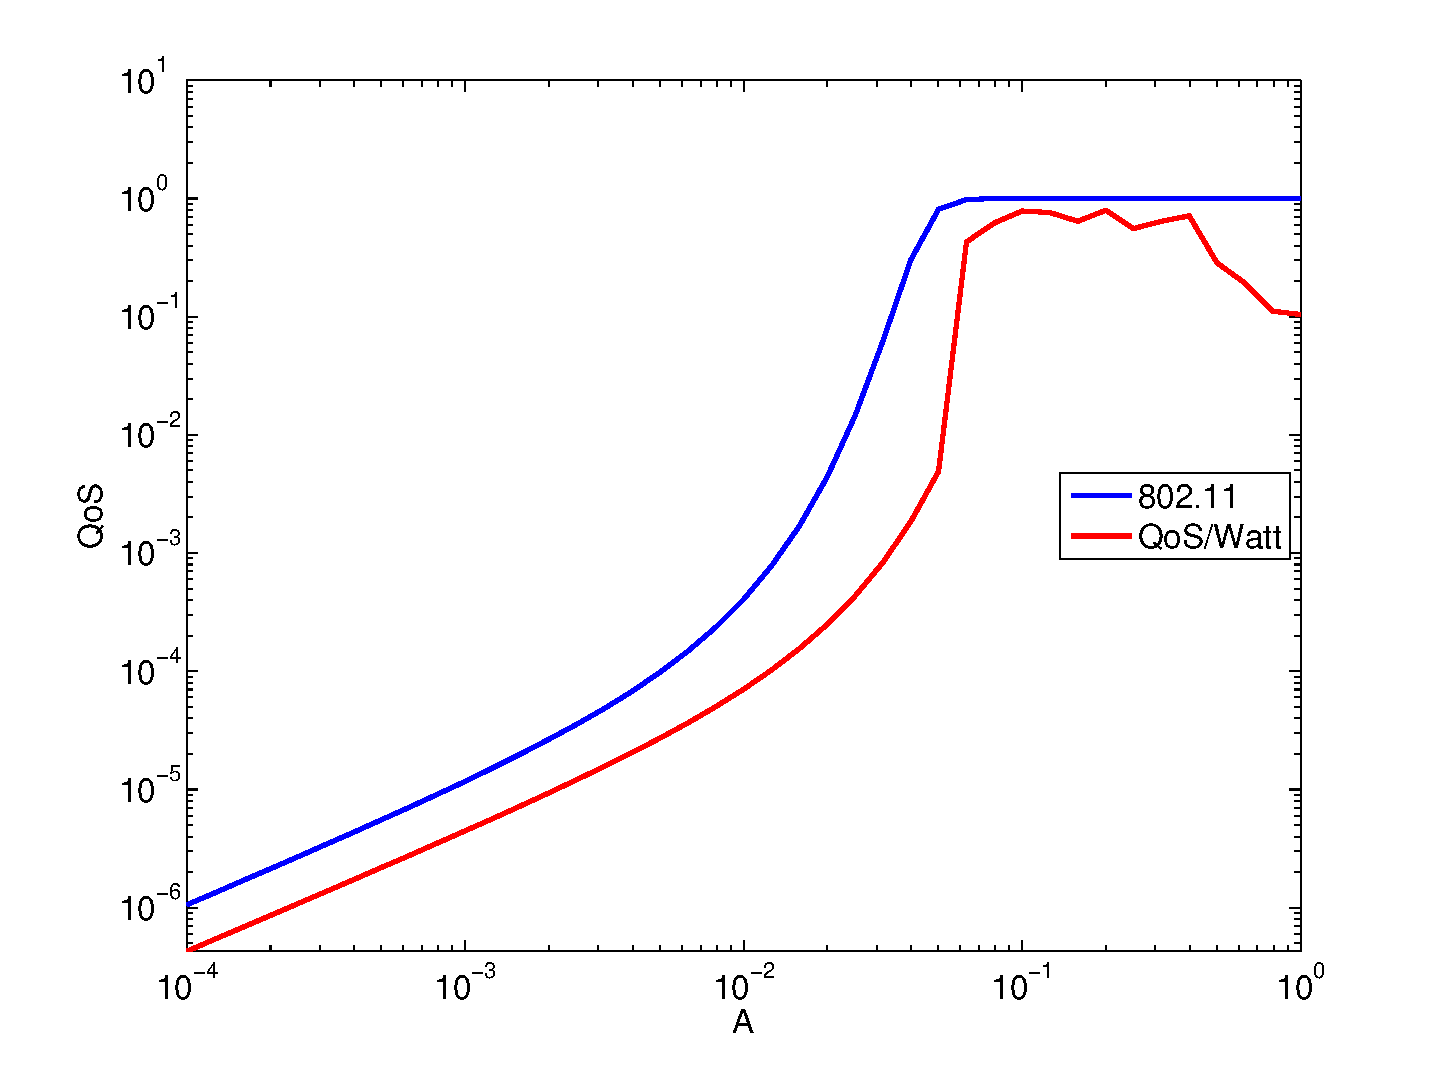
\includegraphics[width=3in]{sim2b.pdf}
\caption{QoS vs. A}
\label{fig:sim2b}
\end{center}
\end{figure}
%
\begin{figure}[htp]
\begin{center}
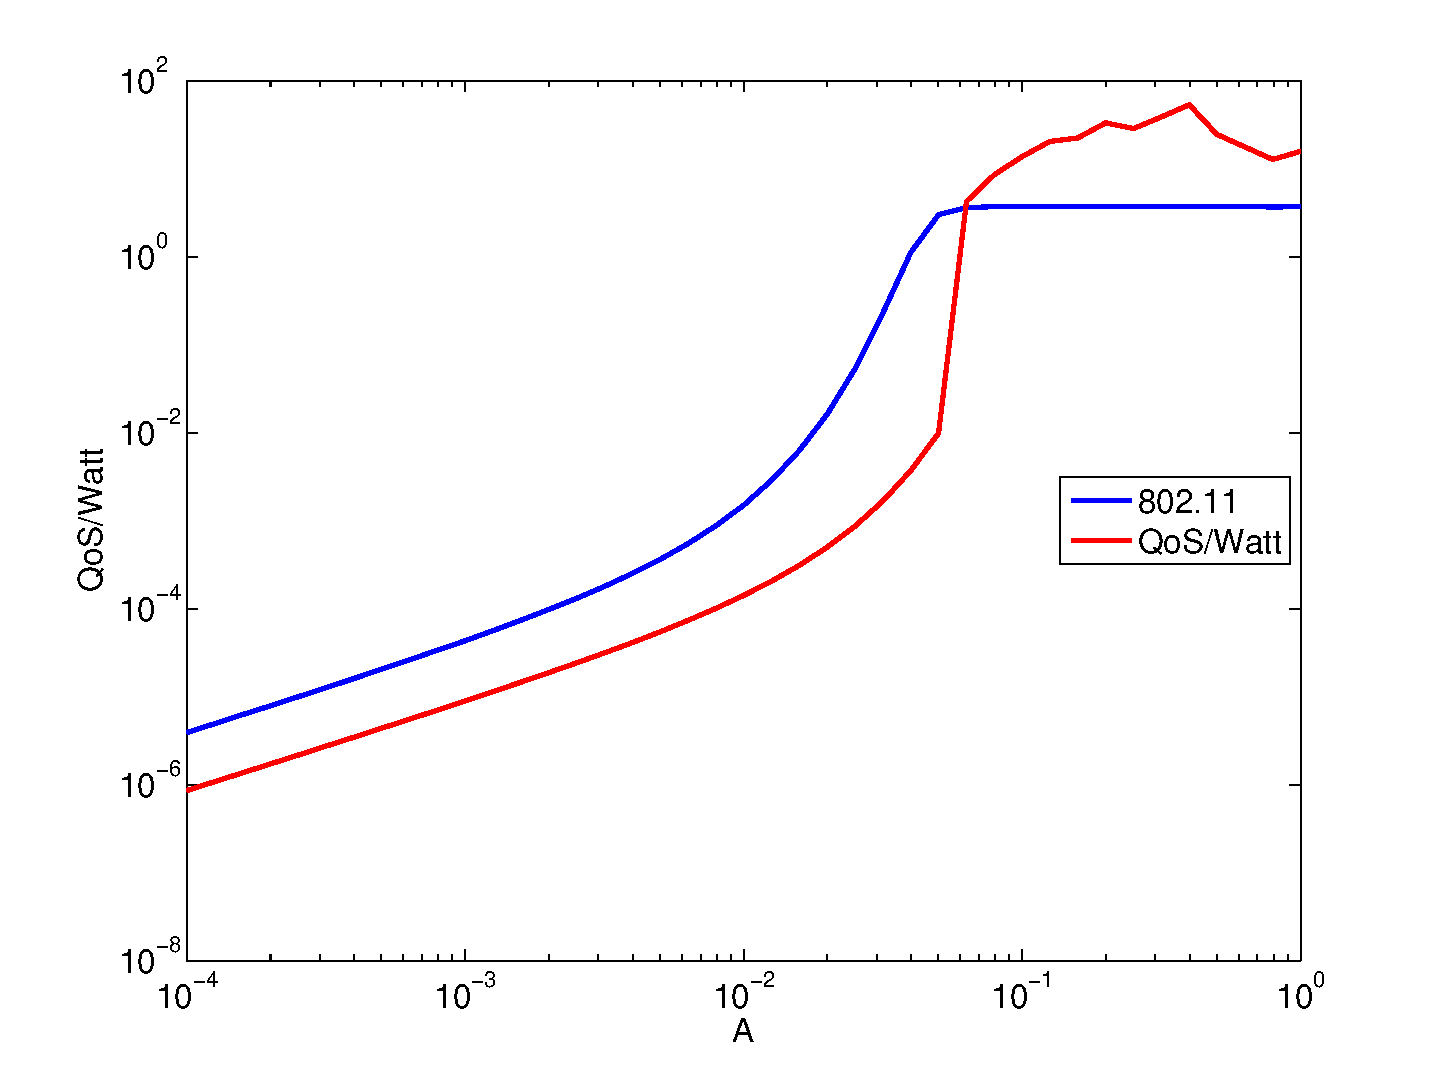
\includegraphics[width=3in]{sim2c.pdf}
\caption{Efficient QoS vs. A}
\label{fig:sim2c}
\end{center}
\end{figure}

Figures \ref{fig:sim2a} and \ref{fig:sim2b} suggest that with regard to throughput or QoS the semi-cooperative appraoch in 802.11 is very beneficial. However, Figure \ref{fig:sim2c} suggests that within some regime of application demand, a selfish utility based on energy efficiency could provide gains in efficiency over 802.11.
%\subsection{Implications Towards Uniqueness: Placement of Peak}
%plot of different uniqueness cases\\

\section{Continuing Work}
In this report, we have shown two of our results:
\begin{itemize}
  \item A selfish behavior-driven utility function, describing QoS tempered by energy consumption
  \item Simulations demonstrating performance of the network
\end{itemize}

We intend to continue our analysis of this utility function to determine conditions for uniqueness and characteristics of equilibria, as well as studying the regimes where this utility definition may prove beneficial.

Furthermore, computation of these results have all relied upon the fact that the persistence probabilities $p_i$ of all users are known throughout the network.  In a realistic protocol this information must be gained by each node either implicitly or explicitly. With a view to doing full resource accounting, the second piece of this project will address the issue of providing various approximations of the $p_i$ to nodes in the network, and exploring the behavior of the solution when differing levels of accuracy are provided.

\bibliographystyle{IEEEtran}
\bibliography{IEEEabrv,elec537proj,books}
\end{document}
